\documentclass[12pt, two column]{article}

\usepackage{fullpage}
%\usepackage[margin=0.5in]{geometry}
\usepackage{enumitem}
%\usepackage{multicol}
\usepackage{csquotes}
\usepackage{natbib}
\usepackage{tabto}
\usepackage{hyperref}
\usepackage{amsmath}
\usepackage{amssymb}
\usepackage{graphicx}

\title{Exploring the Motion Manifold for an Articulated Arm}
\author{ Avikalp Kumar Gupta \& Amitabha Mukerjee}
% \institute{Computer Science and Engineering, IIT Kanpur}

\begin{document}
\maketitle
 
\textbf{\large{Abstract}}\vspace{0.4em}\\
This project is a step towards the extension of visual motion planning algorithms (specifically Debojyoti Dey's M.Tech. thesis work [\cite{deb}]) to 3 dimensions. In this project, we try to generate the \textit{motion manifold} of an articulated arm using only \textit{visual input}. The articulated arm considered in this project has 3 revolute joints, and hence has 3 degrees of freedom.

We use a simulation environment with 3 cameras (vision sensors). Hence, each individual configuration of the robot is expressed as a set of 3 images. We call this set of images, or the configuration it represents, as a \textit{pose} of the robot. A graph is generated over these poses by connecting \textit{k-nearest neighbours} for each pose. The distance between two poses is measured as the Euclidean distance between the pixel values. This graph is supposed to represent the motion manifold of the robot. 

When the graph is constructed over the joint angles, it results in a motion
manifold (a thick hollow cylinder, $\mathbb{R}^2 \times S^1$) as expected.  The visual manifold is
corrupted owing to similarity between distant poses, and results in
\textit{short-circuits}.  The phenomena are discussed and possible approaches to
overcoming it are proposed. 

\section{Introduction}

Our ultimate aim is to plan paths of multiple robots.
Debojyoti had developed a roadmap composition technique in multi-robot environment. Key traits of the algorithm:
\begin{itemize}
  \setlength\itemsep{0em}
  \item \textit{decoupled} motion planning (much more efficient than \textit{centralized} motion planning in terms of time)
  \item oblivious to configuration parameters (The algorithm is implemented on a visual configuration space, and hence is a \textit{generic} method)
  \item probabilistically resolution \textit{complete}
  \item Space optimality: \textit{neighbourhood product lattice} used so that Cartesian products of individual roadmaps are dynamically generated.
\end{itemize}
This algorithm was able to plan paths for 2-D robots.

\textit{``Traditionally, the problem has been handled using a configuration space defined in terms of \textbf{motion parameters} of the robots. An example of such motion parameters are joint angles of an articulated arm. In this work we propose a novel approach based on \textbf{visual input} alone. Such a model works on a random sample set of images of the robots without knowing the motion parameters concerned."}[\cite{deb}]\\
Even though the vision based model makes the algorithm more generic with respect to robots, it raises issues regarding the information captured. Debojyoti implemented the model for 2-D robots. In 2 dimensions, all the instantaneous information about all the objects in the environment can be captured by a single photograph. This includes the complete configuration of the robot. The same is not true in 3 dimensions.

The need of images of the environment from multiple views is obvious. Although, the number of cameras that will be sufficient to capture the \textit{complete} information about the environment depends on the environment itself because \textit{occlusion}, which depends on the geometries of the robots and the objects, can give rise to incompleteness. Algorithms, which can generate the a 3D image using a scan through the environment \cite{bica}, can be used to solve this problem in the future.

\subsection{3-D Articulated Arm}

Since we wanted our method to operate on only visual input, hence we moved forward to work on an algorithm, which might not always be able to find a path, if there exists one, but will only output \textit{correct and collision-free} paths. We started with a 3-D articulated arm with 3 revolute joints (3R) as shown in the figure \ref{3dof}. We installed 3 cameras at orthogonal positions in the environment, which will capture the visual input for our algorithm.

\begin{figure}[h]
  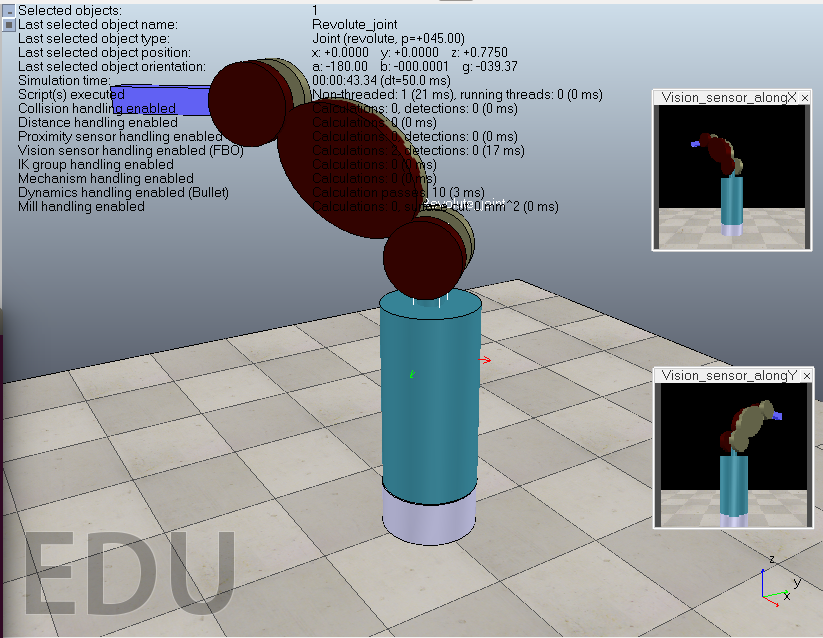
\includegraphics[width=\columnwidth]{graphics/3dof}
  \caption{Robotic arm with 3 revolute joints - Created in v-rep. The 3 smaller windows show the image captured by the vision sensors installed in the scene \textit{\small{(image has been generated using v-rep software)}}}
  \label{3dof}
\end{figure}

This project uses \textit{v-rep} for object modelling and simulation in 3 dimensions. The arm has been created in the \textit{v-rep} environment, and all data, including joint angles' information used for validation, is extracted using the \textit{remote API} functions provided by v-rep. The code for this project is written in \textit{Python} using multiple libraries, including some created by M.S.Ramiah, IIT Kanpur. Stanford's MATLAB code for ISOMAP was used for visualizing the lower dimensional manifold of the images.

\section{Data Generation}
One of the problems, to begin with, is the data generation. In debojyoti's work, the images, which were used to generate the roadmaps for each robot, were generated in the following manner:
\begin{figure}
  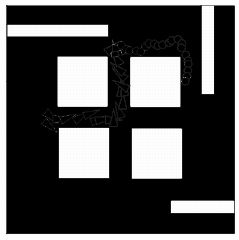
\includegraphics[width=0.45\linewidth]{graphics/exp1_deb}
  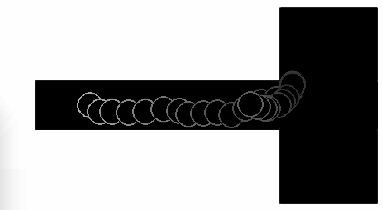
\includegraphics[width=0.45\linewidth]{graphics/exp2_deb}
  \caption{Examples of arenas for Debojyoti's code: Black implies free area and white means obstacle. \textit{Image Source: Grayscaled (to highlight the arena) versions of images from [\cite{deb}]}}
  \label{twoD_arenas}
\end{figure}
\begin{enumerate}
  \item An image file, similar to the ones illustrated in figure \ref{twoD_arenas}, represented the arena.
  \item A position on the arena is chosen at random (and an orientation is also chosen at random) to place the robot objects.
  \item Images are validated on the basis of collision with obstacles. Hence, an image, in which any pixel of the robot coincides with any white pixel, will be rejected.
  \item Each of the remaining image represents a valid pose of the robot in consideration.
\end{enumerate}

And for the articulated arm:\\ \textbf{[Ask and write here]}


\subsection{Image Validation}
We have to capture images of the environment using cameras and use the information from \textit{all the images} to extract information. While generating the set of valid poses, for example, if we want to check collision, we have to go through all the images: the pose is valid if there is \textit{atleast} one image in which the objects are not colliding.

But it turns out that we can never have enough (fixed) cameras. Consider the figure \ref{difficulties}. The environment, in this case, consists of 5 cameras, strategically placed at orthogonal positions to capture maximum information about the scene. The environment does not have any collision, but still all the cameras together are unable to classify this pose as valid.\\
\begin{figure}
  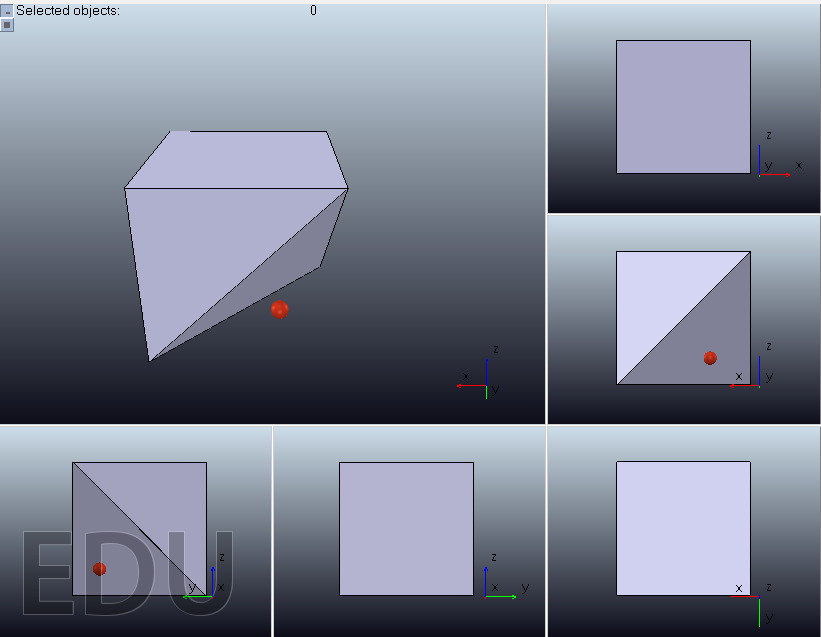
\includegraphics[width=\columnwidth]{graphics/difficulties}
  \caption{(left-top)A small sphere near a truncated cube; (others) all 5 cameras (placed at orthogonal positions) detect ``false" collision \textit{\small{(image has been generated using v-rep software)}}}
  \label{difficulties}
\end{figure}

Apart from the genericness, the paper also describes the closeness of the vision based model to humans:\\
\textit{``Human beings do not appear to use global coordinates; instead, motion is encoded (both consciously and implicitly) in terms of relative poses. Mammals navigating in familiar environments acquire ``place cells" which indicate their position in space, but these are organized in a system of neighbouring columns in the brain that encode nearby places. Thus, the representation appears to encode space in terms of nearby positions rather than a global coordinate."}[\cite{deb}]
%This motivates us to use body-fixed cameras.

\section{Idea/Approach}
  The approach is similar to Debojyoti's work, which includes the following steps:
  \begin{enumerate}
    \item Generate images for a particular pose of a robot from multiple cameras. Repeat for $n$ poses.
    \item Ensure the validity of these poses, i.e. handle \textit{``static collision"}
    \item Create a graph using these poses (described by the set of images corresponding to the same motion parameter values)
    \item Assign weights to the edges of the graph using some metric, preferably distance between the poses
    \item Based on these weights, using K-nearest neighbours for each pose, create a graph which represents the manifold.
    \item Construct a road-map from the initial to the final pose (Shortest paths in the above graph).
    \item Repeat the above steps for all the robots in the scene
    \item Create a composite roadmap using the roadmaps of all the robots (this includes handling \textit{``dynamic collisions"})
  \end{enumerate}

\subsection{Graph Generation}
  \begin{enumerate}
    \item A single set of images for the static obstacles will be captured.
    \item Each robot will be simulated in an independent environment. Random \textit{target angles} for all joints will be given during the simulation, and images will be captured when the robot becomes stable. Simulation will be done to avoid impossible poses (figure \ref{impossible_image}). \\ \textbf{Drawback}: Reduction in the uniformity of the randomness as the boundary configurations become more probable than the other configurations (figure \ref{matPlotLib_image}).
    \begin{figure}
    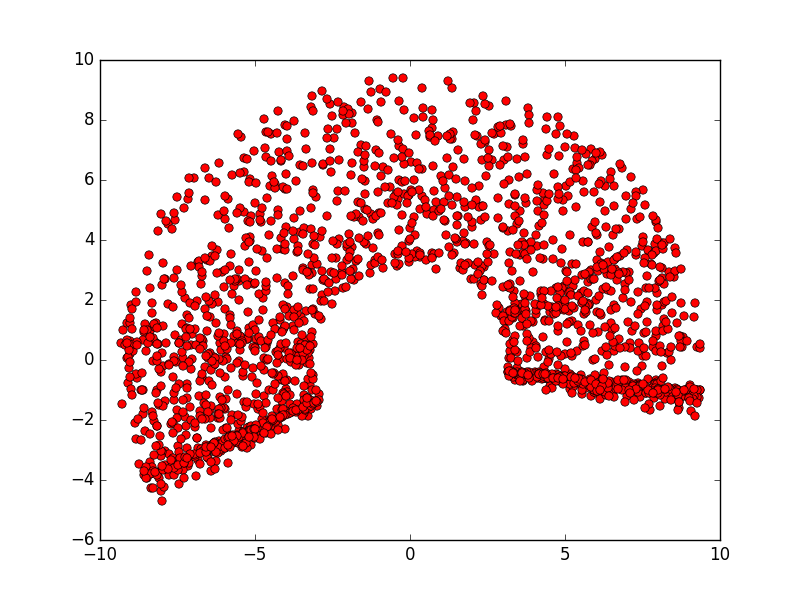
\includegraphics[width=\linewidth]{graphics/theta_2_theta_0}
    \caption{Plot showing accumulation of data points on the boundaries (\textit{Details: Radial distance = $2\pi + \theta_2$, and angle = $\theta_0$})}
    \label{matPlotLib_image}
    \end{figure}
    \item Poses, in which the robot ``seems to be colliding" with some obstacle in \textbf{all} the views, will be rejected. A robot ``seems to be colliding" with some obstacle in a view if for some pixel, the robot's image and the obstacles' image, both have non-zero values in that view.
    \item A \textit{completely connected} graph over all these remaining poses will be created. Each edge will have a weight, based on some metric (eg. distance).
    \item Invalid edges (which lead to collision with obstacles during transition) will be dropped using \textit{local planner}.
    \item K-nearest neighbours for each vertex (pose) will be retained, and rest of the edges will be dropped.
  \end{enumerate}
  This will generate the graph which represents the manifold over which the robot can move.

\subsection{Roadmap Composition}
  After the manifold of the movement of each robot is known, i.e. the above graph is constructed for each robot, we will plan simultaneous paths for the robots from a given initial pose to a given final pose, to minimize, either the total distance travelled by the robots, or the net time taken for the transitions:
  \begin{enumerate}
    \item For each robot, get the shortest paths over the manifolds, from their initial to final poses.
    \item Detect any collision .... \textbf{[see how Debojyoti handles these]}
  \end{enumerate}

\section{Current Progress}
  We have used \textit{v-rep software and API} to generate images [see \ref{v-rep}].
  An external python script was written using v-rep remote API which would:
  \begin{itemize} 
    \item Start the simulation of the currently active scene on the v-rep window
    \item Give random values to the target positions of all the joints
    \item Wait for the robot to reach a stable configuration
    \item Capture the images from each vision sensor, and store the motion parameters for that pose
  \end{itemize}
  Now this script could be used to generate the raw data for any robot [see section \ref{3_DOF_robot} and \ref{ImgGenBaxter}].

\subsection{Choice of a 3-D modelling software}
\label{v-rep}
After going through some 3-D simulation softwares, we chose \textit{v-rep} over the others due to the following:
\begin{enumerate}
  \item Its free version (for educational purposes) supports most of the relevant features
  \item It is a light software and supports 3-D rendering
  \item 3-D modelling is supported inside the software, as well as 3ds-max/blender/CAD can be imported
  \item Objects and simulations can be externally controlled using its remote API for both, C/C++ and Python. (remote APIs for other languages are also supported)
  \item Proper documentation is available, and v-rep is also supported by an online forum
\end{enumerate}

\subsection{Image generation for a robot with 3 dofs (3 revolute joints)}
\label{3_DOF_robot}

The robot in figure \ref{3dof} was made using primitive shapes in v-rep.
It has 3 revolute joints:
One at the base, which makes whole system rotate about $z$-axis. And the other 2 have axes parallel to the $x-y$ plane.
This was created because if you consider the system installed on top of the rotating base cylinder, it is the same R1-R1 articulate arm explained in [\cite{deb}]. Hence we have sufficient knowledge and understanding of its behaviour.

\subsubsection{Manifold}
  As we know, the C-space of the system on top of the base cylinder would be a toroid ($T^2$), if there were no restrictions on the angles which were achievable by the joints. But since both of the top 2 revolute joints cannot rotate $360^\circ$, hence the configuration space is homeomorphic to $\mathbb{R}^2$ space, i.e. a rectangle.

  The base revolute joint can rotate $360^\circ$, and hence is an $S^1$ joint. Hence we expect the C-space of the complete robot to be a ring-like structure (see figure \ref{hollow_cyclinder}).

  \begin{figure}
  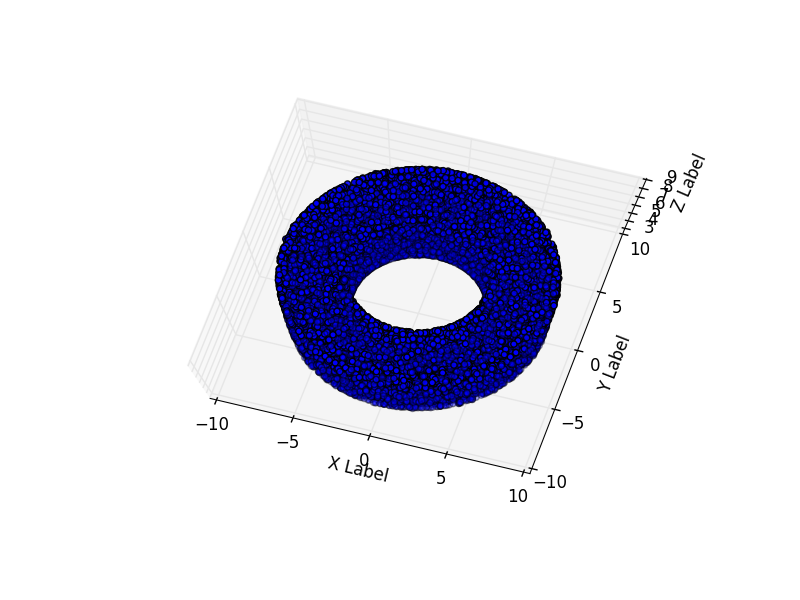
\includegraphics[width=\linewidth]{graphics/hollow_cylinder}
  \label{hollow_cylinder}
  \caption{3-D plot of $\theta_0, \theta_1$ and $\theta_2$ is a hollow cylinder (\textit{Details: $2\pi+\theta_0$ = distance from z-axis, $2\pi+\theta_1$ = distance from x-y plane \& $\theta_2$ = angular displacement along z-axis})}
  \end{figure}

  Unfortunately, this is not what we get in our first attempt. Figure \ref{manifold_visualization} illustrates the manifold of movement obtained on the graph generated on the images. You can observe this as the expected graph with short-circuits.

\subsubsection{Difficulties}
  The following were the major reasons of these short-circuits:
  \begin{itemize}
    \item a jump when 2nd link and the base cylinder are in the same spatial region.
    \item the opposite faces of the middle link get inter-changed ($\theta_1$ change by $180^o$, and $\theta_2$ and $\theta_3$ change signs.
  \end{itemize}

\subsubsection{Proposed solutions}
  The solution of the first problem is to distinguish the different ends of the $3^{rd}$ link using different colors (figure \ref{new_3dof_image}).\\
  The 2nd problem was a fore-seen problem, and it was expected that if we use different colors for the 2 different sides of the middle link, we will be able increase the distance between them. But it turns out that this distance did not increase by much.

\begin{figure}
  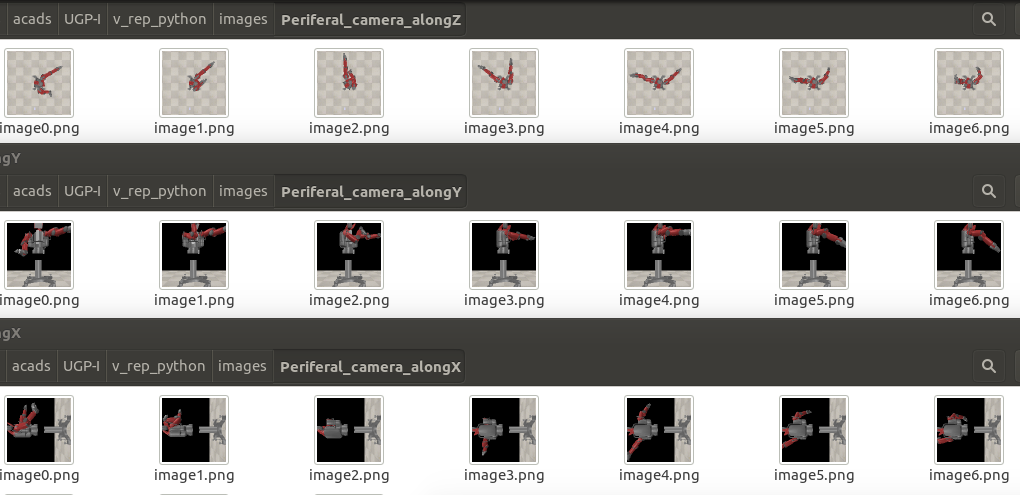
\includegraphics[width=\columnwidth]{graphics/Baxter}
  \caption{An external python script (which uses v-rep remote API) captures images from various peripheral cameras. Images with the same name belong to the same pose.}
  \label{Baxter}
\end{figure}

\section{Future Work}
For the direct extension of Debojyoti's work, the first thing to do now is to complete the remaining steps.\\ But it is quite evident that, due to occlusion, the results produced by it will not have all the traits which the planar model had. Particularly, the algorithm will not be probabilistically resolution-complete.\\
Hence, now we will proceed by understanding how humans and animals plan their motions. The implementation will be similar to paper by Amitabha Mukerjee and Divyanshu Bhartiya called ``A Visual Sense of Space" [\cite{bica}] in which they have proposed a visual characterization for the complex motions of an unknown
mobile system.

Another method could be using body-fixed cameras for capturing information about the environment (example: the case of Baxter) and making the robot learn to find the shortest path. Some study about the various neural network learning algorithms (deep learning and RNNs (including LSTMs)) was also done during the course of this project to proceed in this direction.


\section{Acknowledgement}
I would like to specially thank Mamidela Seetha Ramaiah, a.k.a. MS Ram who had shared with me some very useful libraries he had developed for processing images and generating graphs over them. He also helped me in understanding concepts related to robotics and manifolds (using Choset's book \cite{choset}).

I would also like to thank Debojyoti Dey for spending some very precious time in explaining his implementation.

Lastly, I would like to thank Prof. Amitabha Mukerjee, who is the superviser of the project, for his guidance and expert advice through the project.

%\section{References}
% \bibliographystyle{unsrt}
%\bibliographystyle{alpha} 
\bibliographystyle{apalike} % AWESOME

 \bibliography{report_ref}

\end{document}
